\clearpage
\section{Ellipsoidal Objects}
\label{sect:EllipsoidalObjects}

\subsection{Ellipsoid with two equal semi-axis $R$ and semi-principal axes $\nu R$}
\label{sect:Ellipsoid_ii} ~\\


\begin{figure}[htb]
\begin{center}
%\includegraphics[width=0.706\textwidth,height=0.346\textwidth]{Elpsminr.png}
\includegraphics[width=0.5\textwidth,height=0.245\textwidth]{../images/form_factor/Ellipsoid/Elpsminr.png}
\end{center}
\caption{Ellipse, showing major and minor axes and parameters $a$ and $b$}
\label{minormajoraxes}
\end{figure}

An ellipsoid is a quadric surface in three dimensions obtained by
rotating an ellipse about one of its principal axes. Three
particular cases of an ellipsoid are:
\begin{itemize}
\item If the ellipse is rotated about its major axis, the surface is a prolate spheroid.
\item If the ellipse is rotated about its minor axis, the surface is an oblate spheroid.
\item If the generating ellipse is a circle, the surface is a sphere.
\end{itemize}

\begin{figure}[htb]
\begin{center}
\begin{minipage}[b]{0.5\linewidth}
\begin{center}
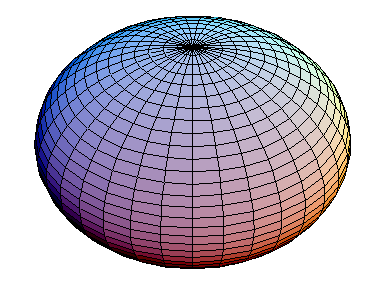
\includegraphics[width=7.5cm,height=5.7cm]{../images/form_factor/Ellipsoid/OblateSpheroid.png} \\
(a) oblate spheroid ($\nu <1$)
\end{center}
\end{minipage}%
\begin{minipage}[b]{0.5\linewidth}
\begin{center}
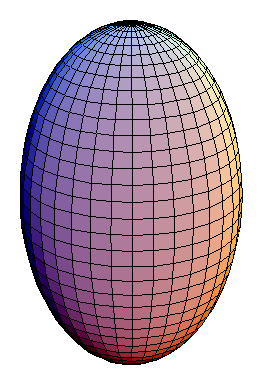
\includegraphics[width=5.1cm,height=7.5cm]{../images/form_factor/Ellipsoid/ProlateSpheroid.png}\\
(b) prolate spheroid ($\nu >1$)
\end{center}
\end{minipage}
\end{center}
\caption{A spheroid is an ellipsoid having two equal equatorial semi-axes. If the equatorial
semi-axis are larger than the principal axis the spheroid becomes oblate (a), if they are smaller
it becomes prolate (b) and if they are equal the spheroid becomes a perfect sphere}
\label{prolate oblate}
\end{figure}

\begin{align}
I_\text{ii}(Q,R,\nu) = \left( \frac{4}{3}\pi R^3 \Delta\eta
\right)^2
 \int_0^{\frac{\pi}{2}}\! K^2\left(Q,R\sqrt{\nu^2\cos^2\Theta+\sin^2\Theta}\right) \sin\Theta\, d\Theta
\end{align}
with $\DS \lim_{Q=0} I_\text{ii}(Q,R,\nu)= \left( \frac{4}{3}\pi
\nu R^3 \Delta\eta \right)^2 $

~\\
\underline{Input Parameters for model \texttt{Ellipsoid ii}:}
\begin{description}
\item[\texttt{R}] radius of the rotational axes
\item[\texttt{nu}]
ratio between radius of the semi-principle axes and equatorial axis.
Values of $\nu<1$ describe a oblate ellipsoid, a value of $\nu=1$ a
sphere, and $\nu>1$ a prolate ellipsoid.
\end{description}

\begin{figure}[htb]
\begin{center}
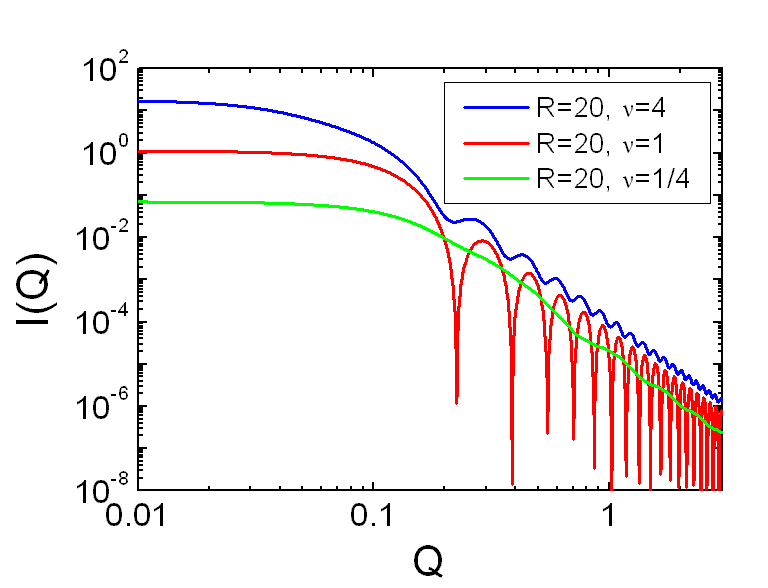
\includegraphics[width=0.768\textwidth,height=0.588\textwidth]{../images/form_factor/Ellipsoid/ellipsoid_ii.png}
\end{center}
\caption{form factor of an ellipsoid with axis $R$, $R$ and $\nu
R$.} \label{fig:I_ellipsoid_ii}
\end{figure}
%%%%%%%%%%%%%%%%%%%%%%%%%%%%%%%%%%%%%%%%%%%%%%%%%%%%%%%%
\clearpage
\subsection{Ellipsoid with two equal equatorial semi-axis $R$ and volume $V$}
\label{sect:Ellipsoid_i} ~\\

\begin{align}
I_\text{i}(Q,R,\nu) = \left( V \Delta\eta
\right)^2
 \int_0^{\frac{\pi}{2}}\! K^2\left(Q,R\sqrt{\nu^2\cos^2\Theta+\sin^2\Theta}\right)\sin\Theta\, d\Theta
\end{align}
with
$$
\nu=\frac{V}{R^3}\frac{3}{4\pi} \quad \mbox{so that}\quad V =\frac{4}{3}\pi\nu R^3
$$
and $\DS \lim_{Q=0} I_\text{i}(Q,R,\nu)= \left(V\Delta\eta\right)^2$

~\\
\underline{Input Parameters for model \texttt{Ellipsoid i}:}
\begin{description}
\item[\texttt{R}] radius of the rotational axes
\item[\texttt{V}] total volume of the ellipsoid.
\end{description}

\begin{figure}[htb]
\begin{center}
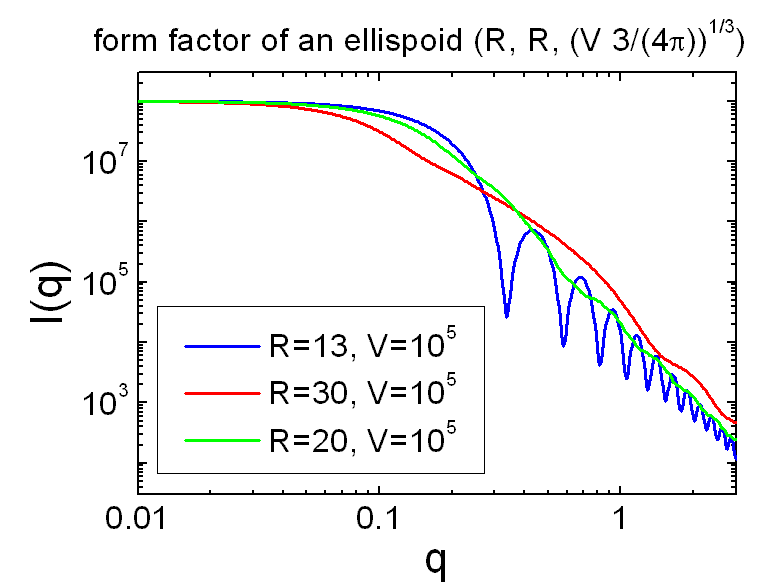
\includegraphics[width=0.768\textwidth,height=0.588\textwidth]{../images/form_factor/Ellipsoid/ellipsoid_i.png}
\end{center}
\caption{form factor of an ellipsoid with axis $R$, $R$ and
$\oldsqrt[3]{V\frac{3}{4\pi}}$.} \label{fig:I_ellipsoid_i}
\end{figure}
%%%%%%%%%%%%%%%%%%%%%%%%%%%%%%%%%%%%%%%%%%%%%%%%%%%%%%%%
\clearpage
\subsection{Ellipsoidal core shell structure}
\label{sect:EllipsoidalCoreShell} ~\\

\begin{figure}[htb]
\begin{center}
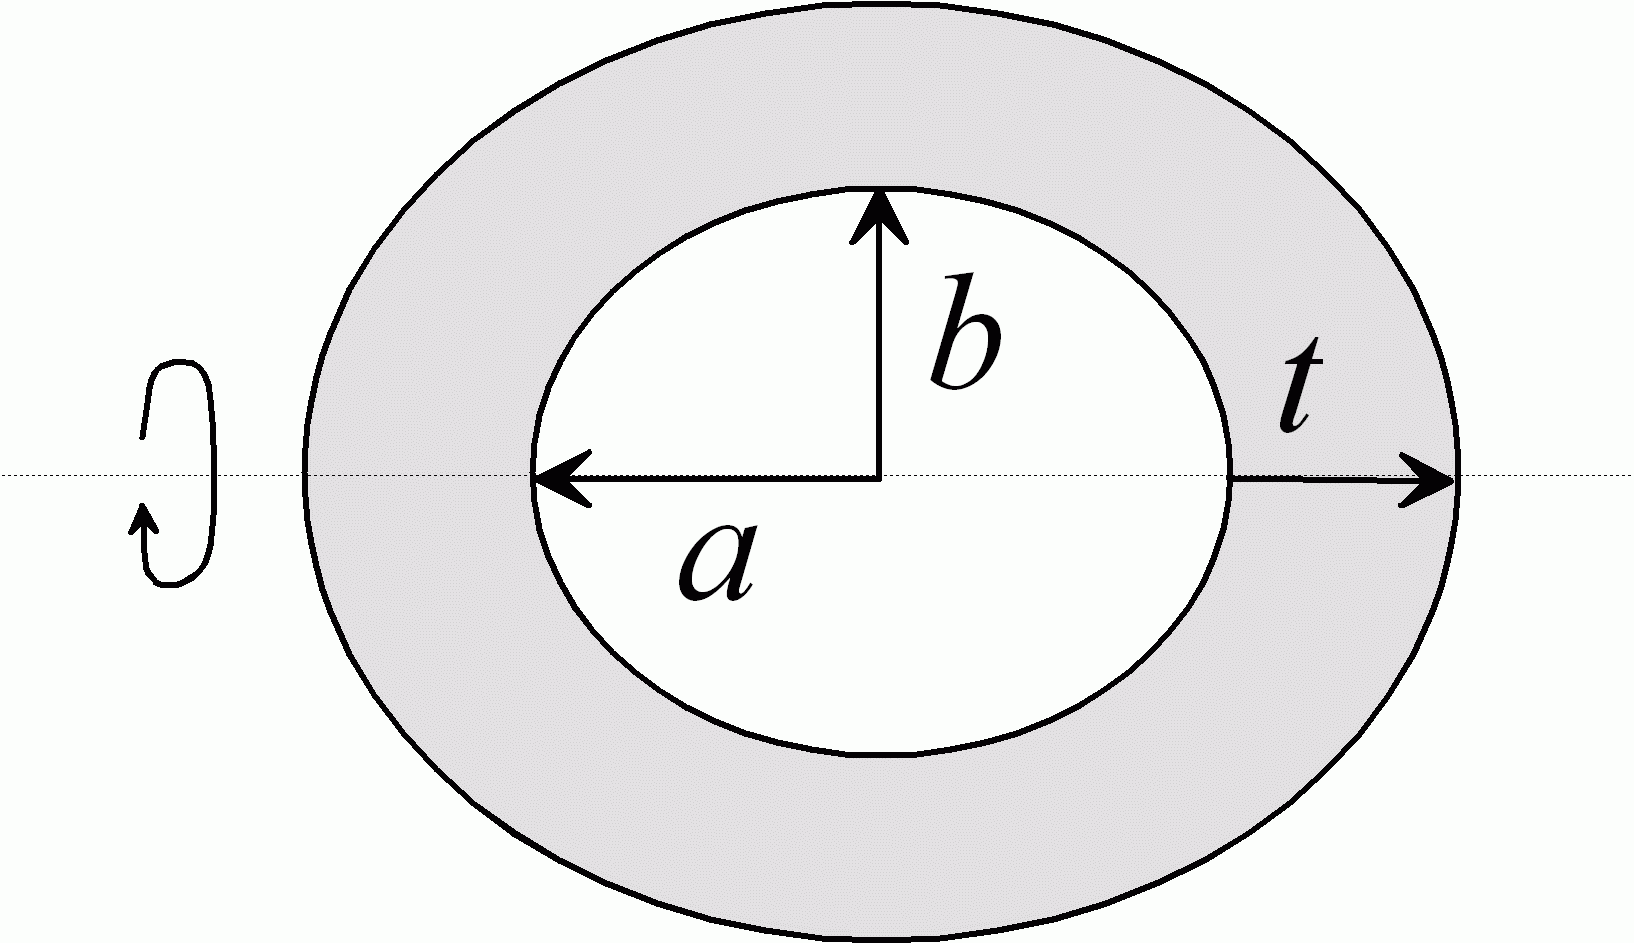
\includegraphics[width=0.5\textwidth,height=0.28855\textwidth]{ellipsoidalShell.png}
\end{center}
\caption{} \label{ellipsoidalShell}
\end{figure}
\begin{align}
I_\text{ECSh}(Q) = \left\langle F^2(Q,\mu) \right\rangle
& = \int_0^1 \left[F(Q,\mu)\right]^2 d\mu \\
\left\langle F(Q,\mu) \right\rangle^2 & = \left[\int_0^1 F(Q,\mu)
d\mu \right]^2
\end{align}
\begin{align}
F(Q,\mu) &= \left(\eta_\text{c}-\eta_\text{sh}\right) V_c\left[
\frac{3j_1(x_c)}{x_c}\right]
          +\left(\eta_\text{sh}-\eta_\text{sol}\right) V_t\left[ \frac{3j_1(x_t)}{x_t}\right]
          \nonumber \\
j_1(x) &= \frac{\sin(x)-x\cos(x)}{x^2} \nonumber \\
x_c &= Q \sqrt{a^2\mu^2+b^2(1-\mu^2)} \nonumber \\
x_c &= Q \sqrt{(a+t)^2\mu^2+(b+t)^2(1-\mu^2)} \nonumber \\
V_c &= \frac{4}{3}\pi ab^2 \nonumber \\
V_t &= \frac{4}{3}\pi (a+t)(b+t)^2 \nonumber
\end{align}
\begin{align}
\eta_\text{c} &: \text{scattering length density of core} \nonumber \\
\eta_\text{sh} &: \text{scattering length density of shell} \nonumber \\
\eta_\text{sol} &: \text{scattering length density of solvent} \nonumber \\
a &: \text{semi-principal axes of elliptical core} \nonumber \\
b &: \text{equatorial semi-axis of elliptical core} \nonumber \\
t &: \text{thickness of shell} \nonumber \\
V_c &: \text{volume of core} \nonumber \\
V_t &: \text{total volume of core along with shell} \nonumber
\end{align}

\vspace{0.5cm}

\underline{Input Parameters for model \texttt{EllipsoidalCoreShell}:}
\begin{description}
\item[\texttt{a}] semi-principal axes of elliptical core $a$
\item[\texttt{b}] equatorial semi-axis axes of elliptical core $b$
\item[\texttt{t}] thickness of shell $t$
\item[\texttt{eta\_c}] scattering length density of core $\eta_\text{c}$
\item[\texttt{eta\_sh}] scattering length density of shell $\eta_\text{sh}$
\item[\texttt{eta\_sol}] scattering length density of solvent $\eta_\text{sol}$
\end{description}

\begin{figure}[htb]
\begin{center}
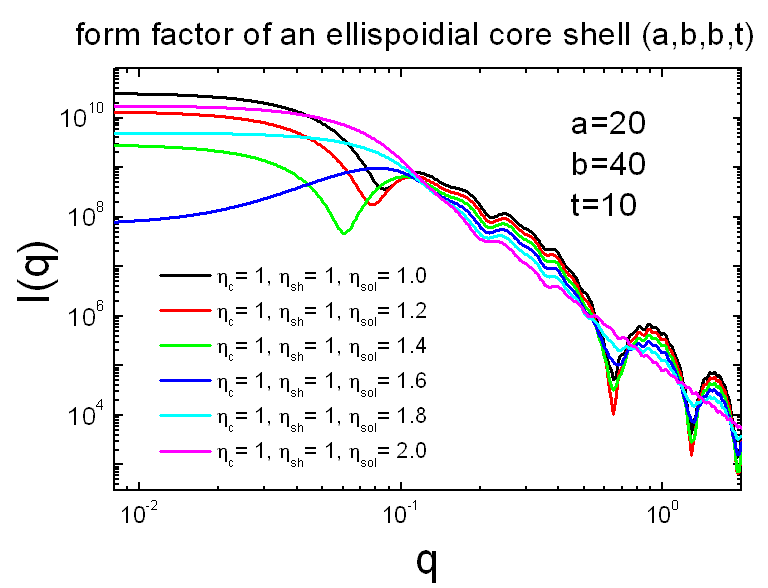
\includegraphics[width=0.768\textwidth,height=0.588\textwidth]{../images/form_factor/Ellipsoid/ellipsoidal_core_shell.png}
\end{center}
\caption{form factor of an ellipsoidal core shell $a$, $b$, $b$ and
$t$.} \label{fig:I_ellipsoidal_core_shell}
\end{figure}
%%%%%%%%%%%%%%%%%%%%%%%%%%%%%%%%%%%%%%%%%%%%%%%%%%%%%%%%
\clearpage
\subsection{triaxial ellipsoidal core shell structure}
\label{sect:triaxEllShell1} ~\\

\begin{figure}[htb]
\begin{center}
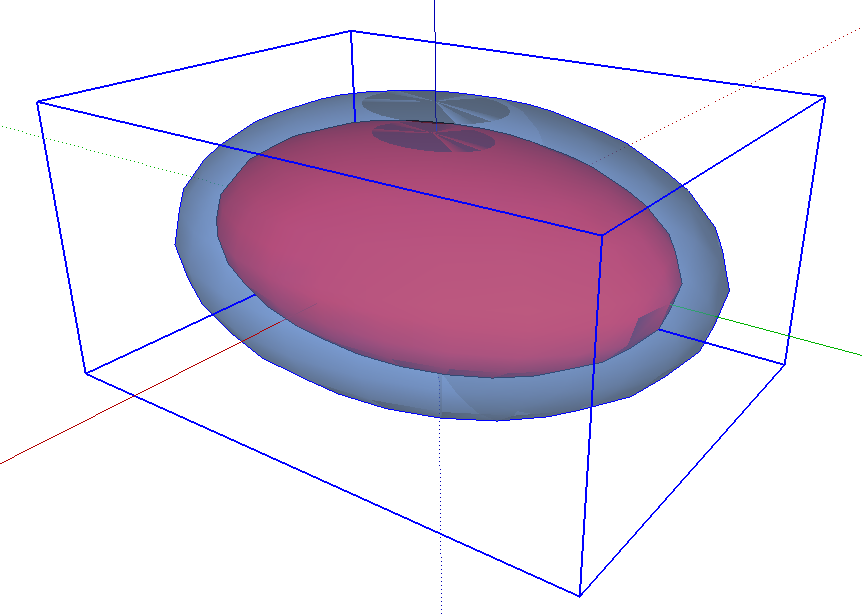
\includegraphics[width=0.45\textwidth,height=0.32177\textwidth]{../images/form_factor/Ellipsoid/triaxEll.png}
\hspace{0.08\textwidth}
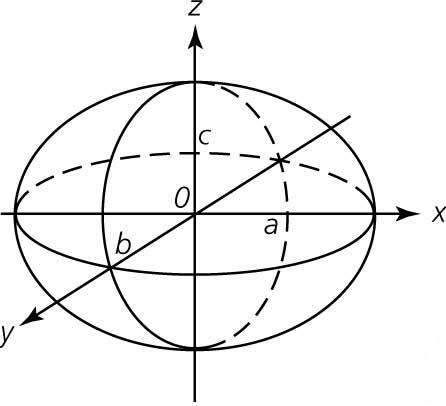
\includegraphics[width=0.45\textwidth,height=0.4096\textwidth]{../images/form_factor/Ellipsoid/A4ellipd.png}
\end{center}
\caption{triaxial ellipsoidal core shell structure} \label{triaEllShell}
\end{figure}

\begin{align}
I_\text{triaxEllSh}(Q) &= \int^1_0 \int ^1_0 dx\,dy\, K_\text{sh}^2(Q,R,R_t)\\
K(QR)         &= 3 \frac{\sin QR - QR\cos QR}{(QR)^3} \\
K_\text{sh}(Q,R,R_t) &= \left(\eta_\text{c}-\eta_\text{sh}\right)K(QR)+\left(\eta_\text{sh}-\eta_\text{sol}\right)K(QR_t) \\
R^2 &= \left[a^2\cos^2\left(\pi x/2\right) + b^2\sin^2\left(\pi x/2\right)\right](1-y^2)+c^2y^2 \nonumber \\
R_t^2 &= \left[(a+t)^2\cos^2\left(\pi x/2\right) + (b+t)^2\sin^2\left(\pi x/2\right)\right](1-y^2)+(c+t)^2y^2
\nonumber \\
V_c &= \frac{4}{3}\pi abc \nonumber \\
V_t &= \frac{4}{3}\pi (a+t)(b+t)(c+t) \nonumber
\end{align}
\begin{align}
\eta_\text{c} &: \text{scattering length density of core} \nonumber \\
\eta_\text{sh} &: \text{scattering length density of shell} \nonumber \\
\eta_\text{sol} &: \text{scattering length density of solvent} \nonumber \\
a &: \text{semi-axes of elliptical core} \nonumber \\
b &: \text{semi-axes of elliptical core} \nonumber \\
c &: \text{semi-axes of elliptical core} \nonumber \\
t &: \text{thickness of shell} \nonumber \\
V_c &: \text{volume of core} \nonumber \\
V_t &: \text{total volume of core along with shell} \nonumber
\end{align}

\vspace{3cm}
\underline{Input Parameters for model \texttt{triaxEllShell1}:}
\begin{description}
\item[\texttt{a}] semi-axes of elliptical core $a$
\item[\texttt{b}] semi-axes of elliptical core $b$
\item[\texttt{c}] semi-axes of elliptical core $c$
\item[\texttt{t}] thickness of shell $t$
\item[\texttt{eta\_c}] scattering length density of core $\eta_\text{c}$
\item[\texttt{eta\_sh}] scattering length density of shell $\eta_\text{sh}$
\item[\texttt{eta\_sol}] scattering length density of solvent $\eta_\text{sol}$
\end{description}

\begin{figure}[htb]
\begin{center}
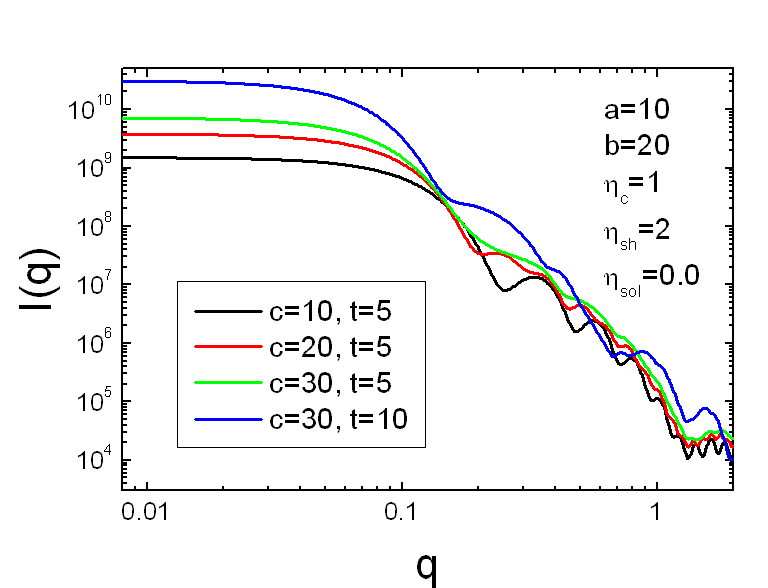
\includegraphics[width=0.768\textwidth,height=0.588\textwidth]{../images/form_factor/Ellipsoid/triax_ellipsoidal_core_shell.png}
\end{center}
\caption{Form factor of an triaxial ellipsoidal core shell with semi
axis $a$, $b$ and $c$ and a shell thickness $t$.}
\label{fig:I_ellipsoidal_core_shell}
\end{figure}
